\documentclass{article}


\usepackage{manualdoprofessor}
\usepackage{fichatecnica}
\usepackage{lipsum,media9,graficos}
\usepackage[justification=raggedright]{caption}




\usepackage{bncc}
\usepackage[youkali]{logoedlab}

 

\begin{document}


% Abertura -----------------------------------------------------------------
										\begin{frame}\begin{raggedleft}
										\Huge 
O peru de natal e outros contos						\\
										\huge 
Mário de Andrade							\\
										\bigskip
										\normalsize
Tema: Ficção, mistério e fantasia		\\	
Gênero: Conto, crônica e novela			\\\vfill\hfill

\publishername

										\end{raggedleft}

\smallskip
\includegraphics[width=2cm]{ccbync.png}\hfill
\end{frame}

% Logo ---------------------------------------------------------------------

\begin{frame}{\textsc{videotutorial do aluno}}
\vspace{-2cm}\begin{figure}
	\IfFileExists{PNLD0028-01.png}{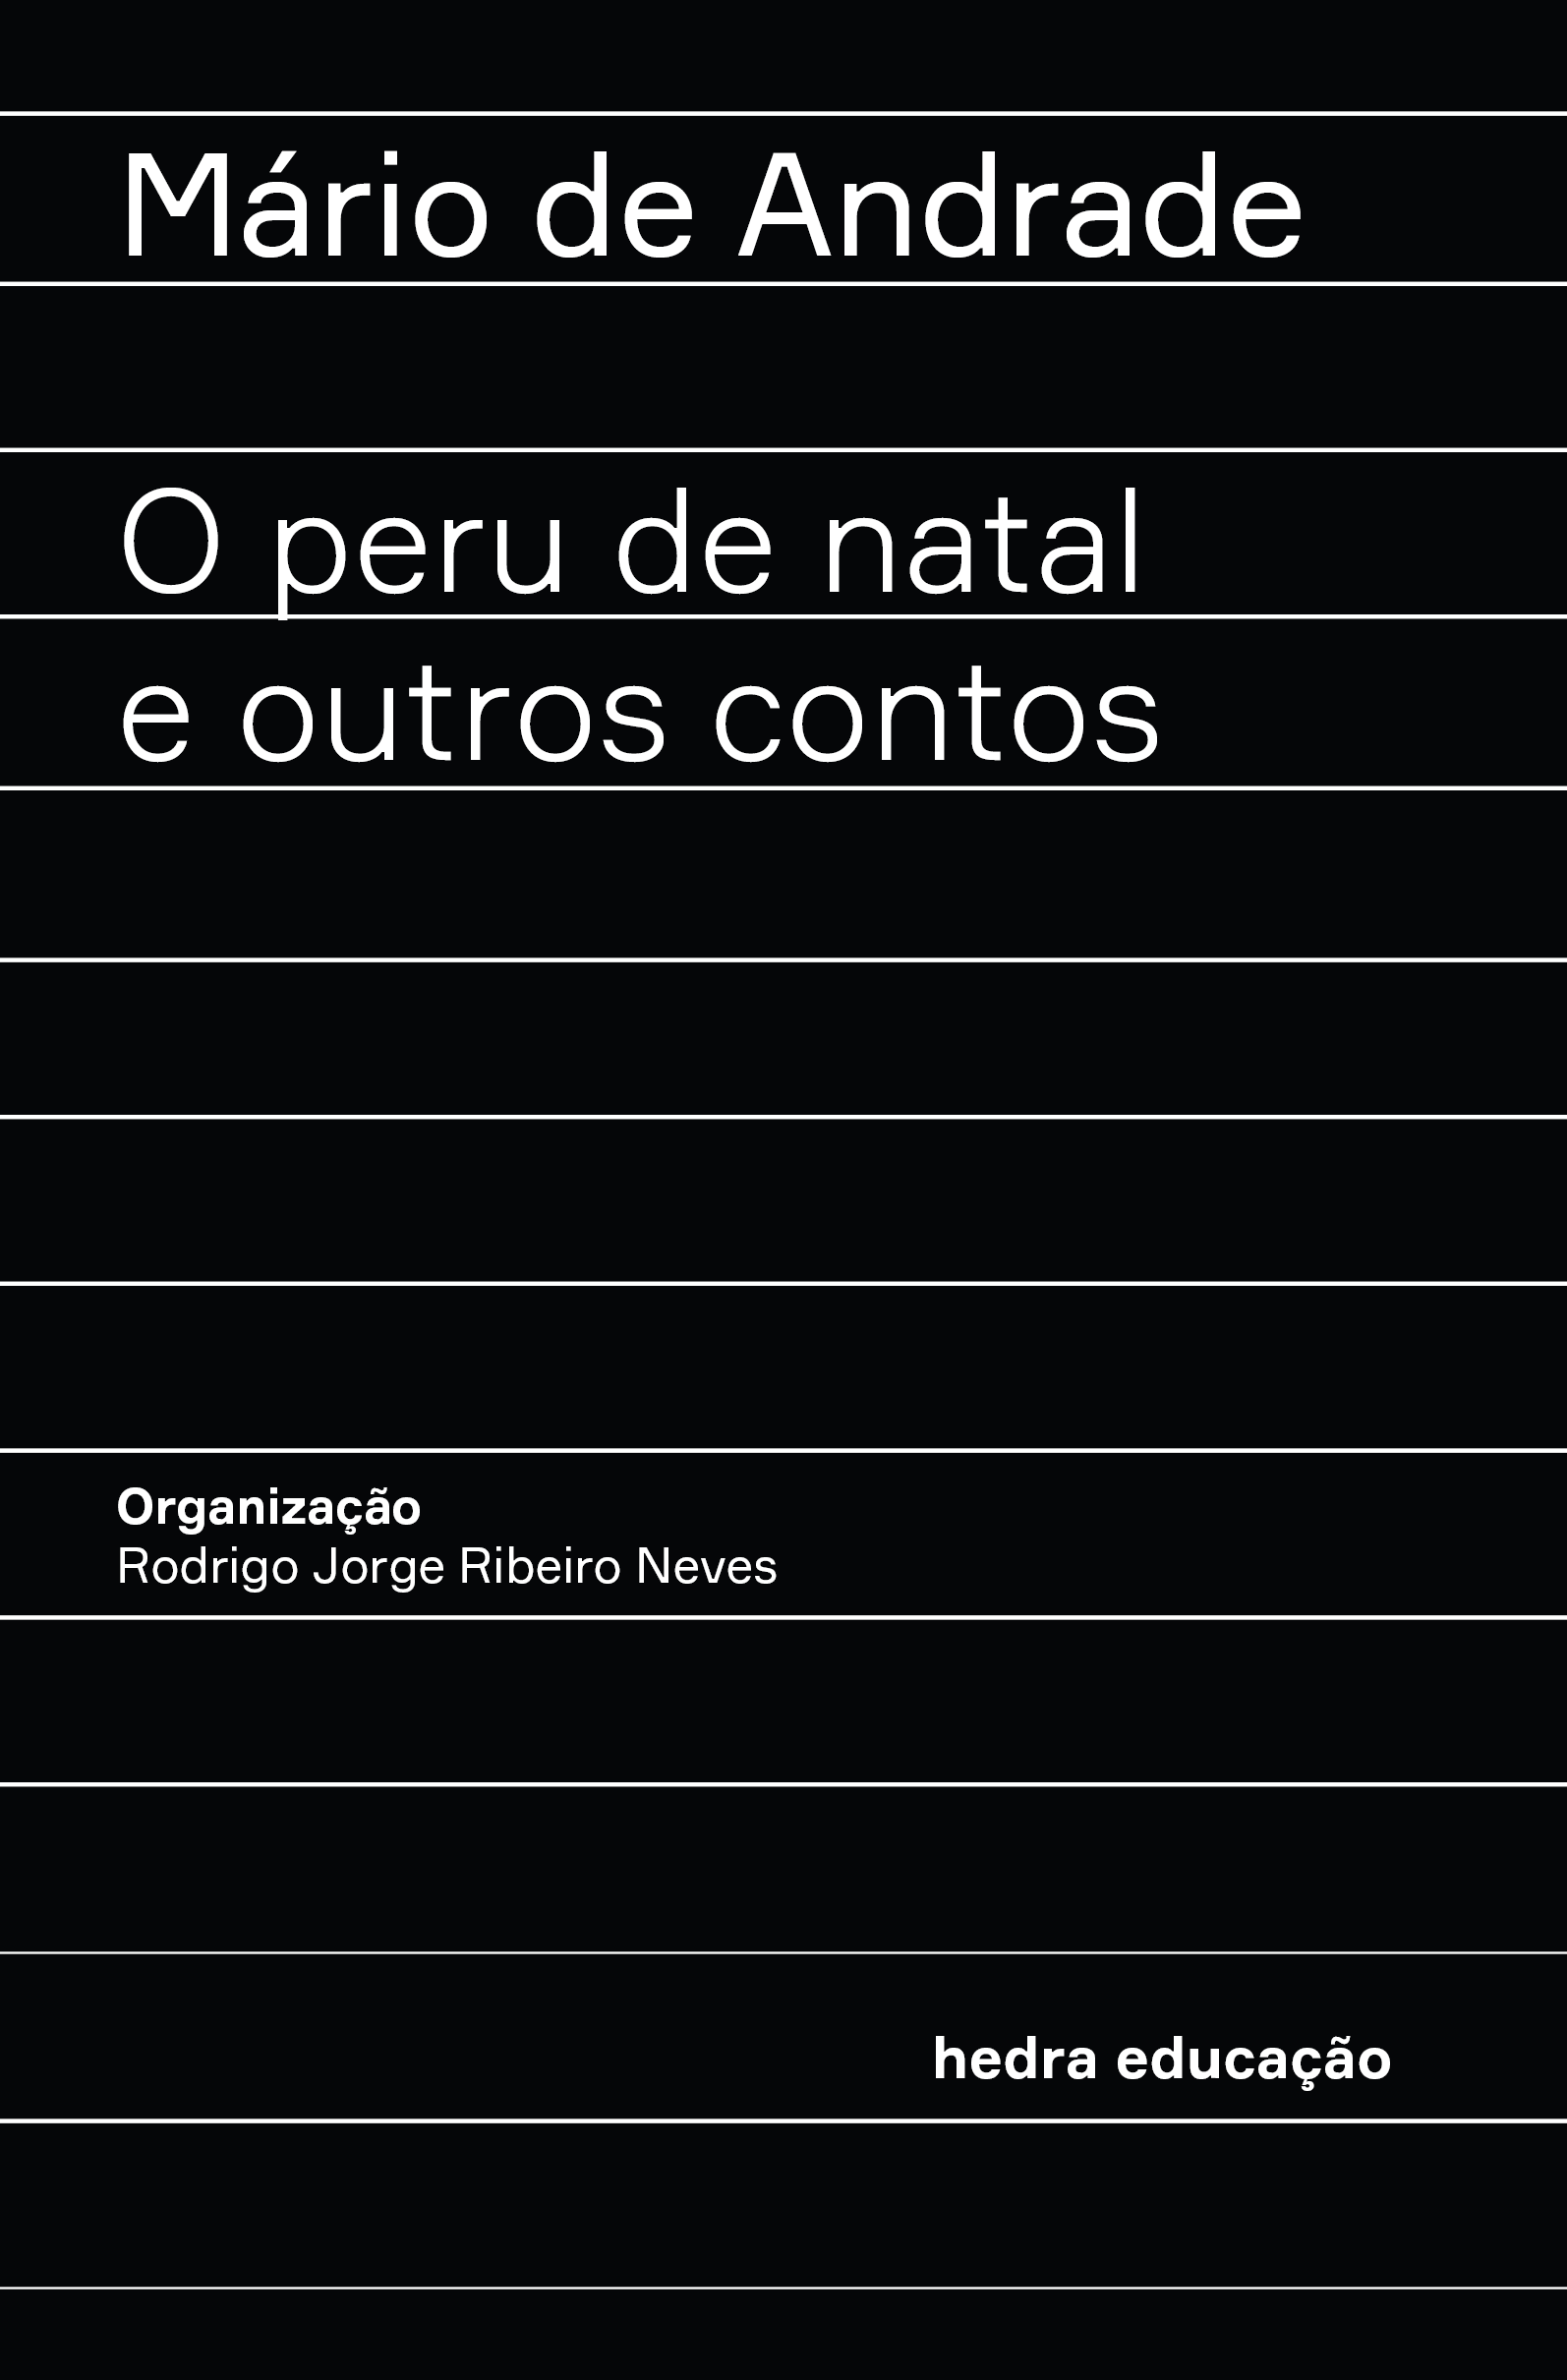
\includegraphics[width=5cm]{PNLD0028-01.png}}{Aplicar Capa!!}
\end{figure}
\end{frame}


% Slides -------------------------------------------------------------------

\begin{frame}
\hfill\Huge
\textsc{sobre obra e autor}
\end{frame}

\begin{frame}
\hfill\Huge
\textsc{sobre o gênero do livro}
\end{frame}

% BNCC ---------------------------------------------------------------------

% \begin{frame}[plain]{Habilidades (BNCC)}
% \vspace{-2cm}
% \BNCC{EM13CHS504}
% \BNCC{EM13CHS601}
% \end{frame}

\setbeamertemplate{background}{%
		\includegraphics[width=\paperwidth, 
		height=\paperheight, 
		keepaspectratio]{BGW.pdf}}
% Fechamento ---------------------------------------------------------------

\begin{frame}
\centering\hfill\includegraphics[width=7cm]{\logoeditora}
\end{frame}

\end{document}
